Examine the marginal and bivariate normality of the observations on variables
$X_{1}$, $X_{2}$, $X_{3}$, and $X_{4}$ for the data in Table 4.3.

For ($x_{1}$), we're sending a shockwave down a board and measuring the board stiffness, and have 30 valid observations. The simulated 0.01, 0.05, and 0.10 level critical correlation coefficient test values for a sample size of 30 are, 0.9488, 0.9647, and 0.9711, respectively. The Q-Q correlation coefficient using the raw data was 0.9599, so the data would not be considered normally distributed at the 0.05 and 0.10 levels.

The transformation suggested by the power transformation was -0.6112, but was rounded to -0.5, so $x_{1}^{\prime} = 1/\sqrt{x_{1}}$. The Q-Q correlation coefficient on the transformed data was 0.9873, which is larger than all the critical values, so the data is now normally distributed at the 0.01, 0.05, and 0.10 levels. Below are the results of the power transformation and the Q-Q plots of the raw and transformed data. The original plot wasn't too bad, with one value with a higher stiffness value than the rest, but the transformed data has brought in the larger value to make the plot much more linear.

\begin{center}
    \begin{figure}[H]
        \centering
        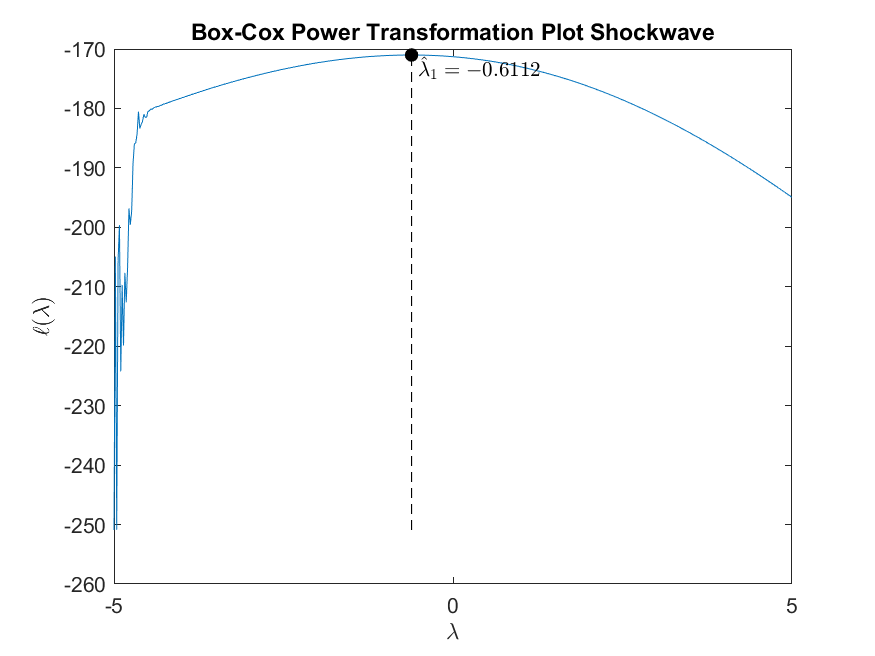
\includegraphics[scale=0.6]{./matlab/chapter-4/sol4.33.power.1.png}
    \end{figure}
\end{center}

\begin{center}
    \begin{figure}[H]
        \centering
        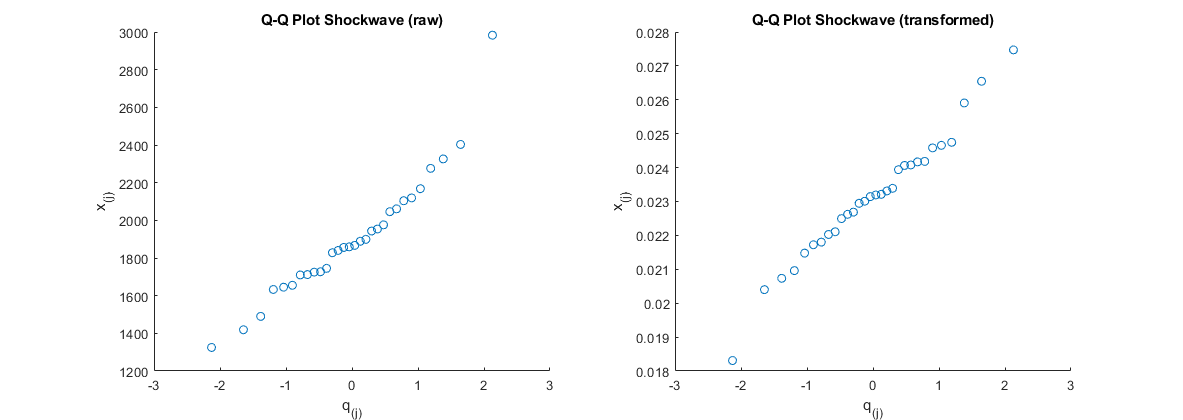
\includegraphics[scale=0.4]{./matlab/chapter-4/sol4.33.qq.1.png}
    \end{figure}
\end{center}

For ($x_{2}$), we're determining the stiffness of a bord while it's being vibrated, and have 30 valid observations. The simulated 0.01, 0.05, and 0.10 level critical correlation coefficient test values for a sample size of 30 are, 0.9488, 0.9647, and 0.9711, respectively. The Q-Q correlation coefficient using the raw data was 0.9504, so the data would not be considered normally distributed at the 0.05 and 0.10 levels.

The transformation suggested by the Box-Cox power transformation was -0.7715, but was rounded to -0.75, so $x_{2}^{\prime} = 1/\sqrt[4]{x_{2}^{3}}$. The Q-Q correlation coefficient on the transformed data was 0.9828, which is larger than all the critical values, so the data is now normally distributed at the 0.01, 0.05, and 0.10 levels. Below are the results of the power transformation and the Q-Q plots of the raw and transformed data. The original plot wasn't too bad, with one value with a higher stiffness value than the rest, just like for $x_{1}$, but the transformed data has brought in the larger value to make the plot much more linear.

\begin{center}
    \begin{figure}[H]
        \centering
        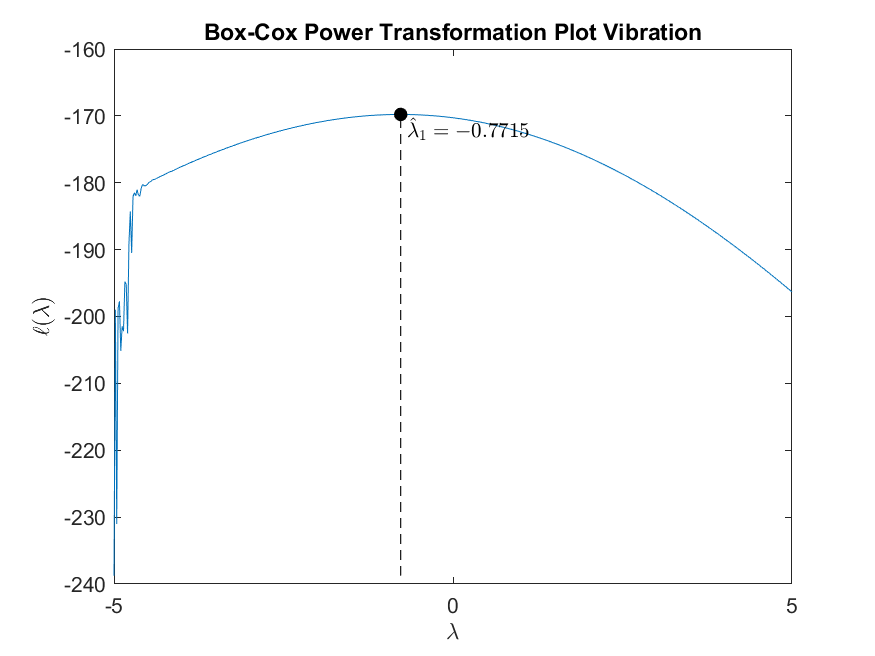
\includegraphics[scale=0.6]{./matlab/chapter-4/sol4.33.power.2.png}
    \end{figure}
\end{center}

\begin{center}
    \begin{figure}[H]
        \centering
        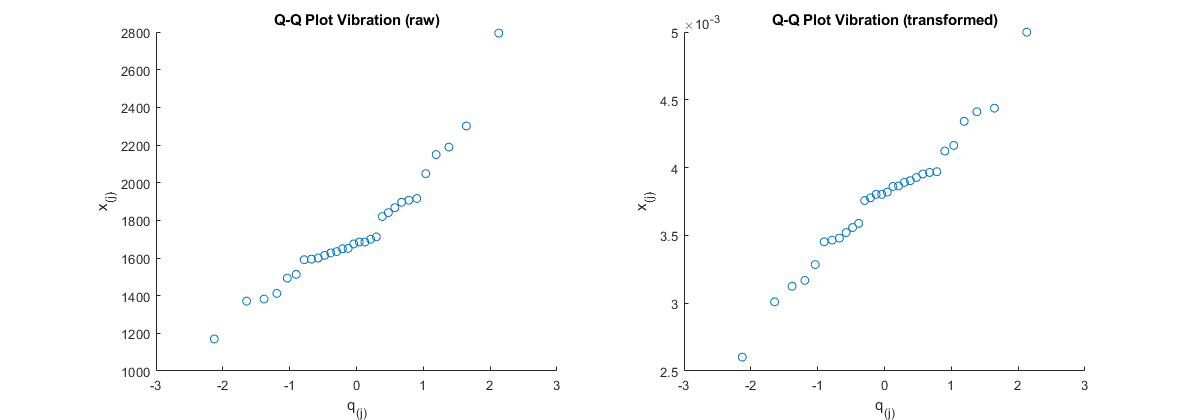
\includegraphics[scale=0.4]{./matlab/chapter-4/sol4.33.qq.2.png}
    \end{figure}
\end{center}

For ($x_{3}$), we're determining the stiffness of a bord in a static test, and have 30 valid observations. The simulated 0.01, 0.05, and 0.10 level critical correlation coefficient test values for a sample size of 30 are, 0.9488, 0.9647, and 0.9711, respectively. The Q-Q correlation coefficient using the raw data was 0.9634, so the data would not be considered normally distributed at the 0.05 and 0.10 levels.

The transformation suggested by the Box-Cox power transformation was -0.7515, but was rounded to -0.75, so $x_{3}^{\prime} = 1/\sqrt[4]{x_{3}^{3}}$. The Q-Q correlation coefficient on the transformed data was 0.9828, which is larger than all the critical values, so the data is now normally distributed at the 0.01, 0.05, and 0.10 levels. Below are the results of the power transformation and the Q-Q plots of the raw and transformed data. The original plot wasn't too bad, with a few values with higher stiffness value than the rest, similar to $x_{1}$ and $x_{2}$, but the transformed data has brought in the larger value to make the plot much more linear.

\begin{center}
    \begin{figure}[H]
        \centering
        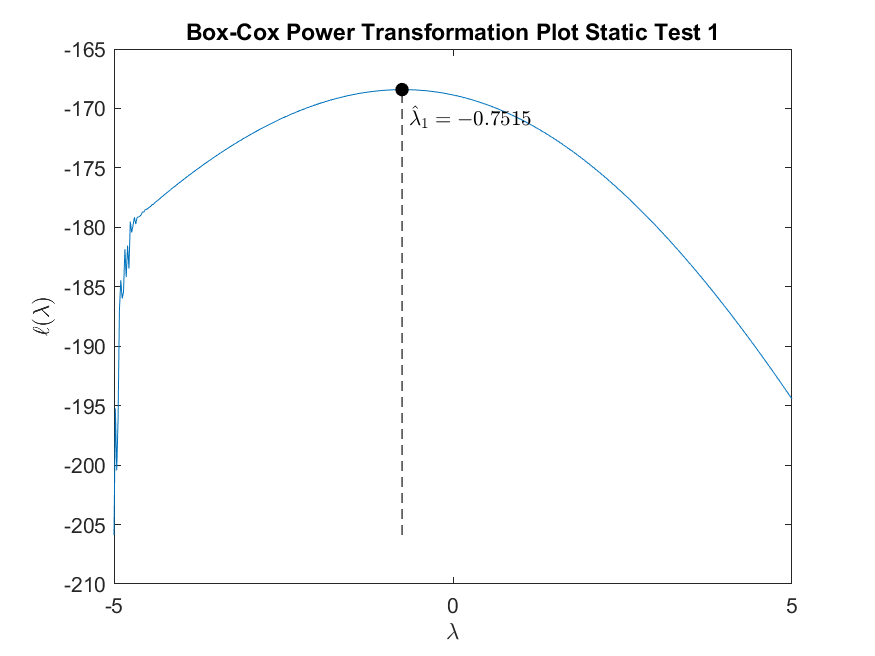
\includegraphics[scale=0.6]{./matlab/chapter-4/sol4.33.power.3.png}
    \end{figure}
\end{center}

\begin{center}
    \begin{figure}[H]
        \centering
        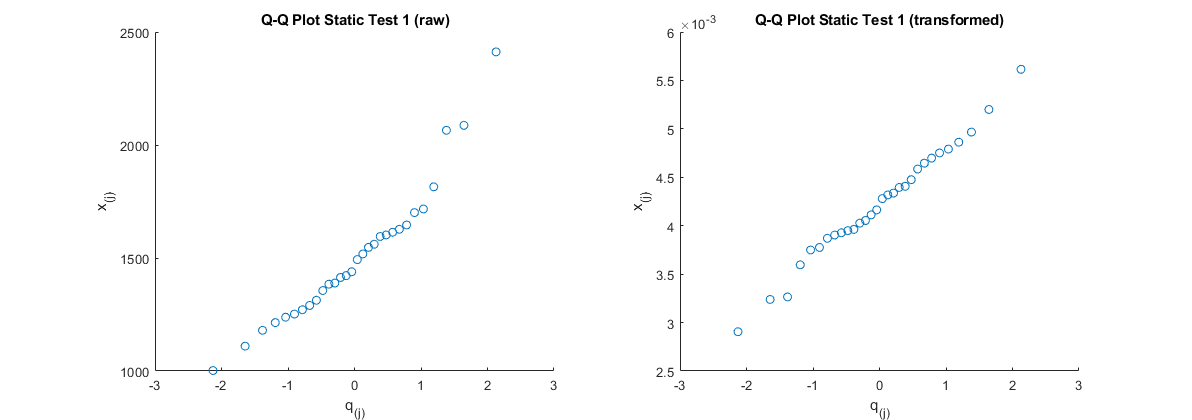
\includegraphics[scale=0.4]{./matlab/chapter-4/sol4.33.qq.3.png}
    \end{figure}
\end{center}

For ($x_{4}$), we're determining the stiffness of a bord in a static test, again, and have 30 valid observations. The simulated 0.01, 0.05, and 0.10 level critical correlation coefficient test values for a sample size of 30 are, 0.9488, 0.9647, and 0.9711, respectively. Our Q-Q correlation value of 0.9803 is larger than all of these, so out data is actually considered normally distributed at all 3 levels. Because of this I won't really bolther displaying the Box-Cox transformation results, but the power transformation of -0.3507 bumps the Q-Q correlation coefficient up to 0.9928. The raw data Q-Q plot is below.

\begin{center}
    \begin{figure}[H]
        \centering
        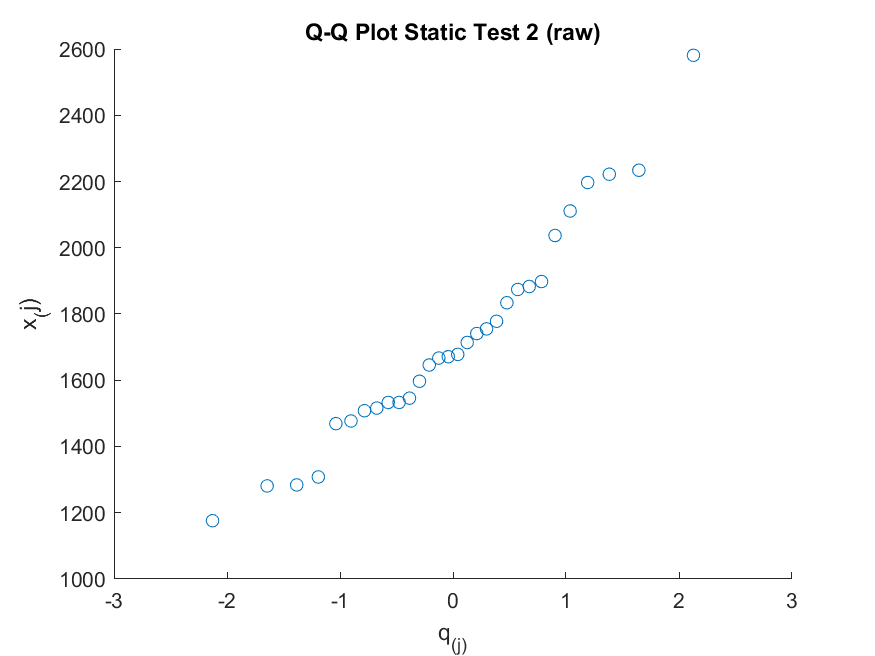
\includegraphics[scale=0.6]{./matlab/chapter-4/sol4.33.qq.4.png}
    \end{figure}
\end{center}

Checking out the bivariate, we have ${4 \choose 2} = 6$ pairs of variables to evaluate for

\[
\left\{
    \begin{NiceArray}{ccc}
        (x_{1}, x_{2}), & (x_{1}, x_{3}), & (x_{1}, x_{4}), \\
        (x_{2}, x_{3}), & (x_{2}, x_{4}), \\
        (x_{3}, x_{4})
    \end{NiceArray}
\right\}
\]

\begin{table}[H]
    \caption*{Proportion less than $\chi_{2}^{2}(0.50) = 1.3863$}
    \centering
    \begin{tabular}{lcc}
        \hline % chktex 44
        Variables & Raw Data & Transformed Data \\
        \hline % chktex 44
        $(x_{1}, x_{2})$ & 0.5333 &    0.5000 \\
        $(x_{1}, x_{3})$ & 0.6333 &    0.6000 \\
        $(x_{1}, x_{4})$ & 0.6000 &    0.6000 \\
        $(x_{2}, x_{3})$ & 0.7000 &    0.6333 \\
        $(x_{2}, x_{4})$ & 0.7000 &    0.6667 \\
        $(x_{3}, x_{4})$ & 0.5667 &    0.6000 \\
        \hline % chktex 44
    \end{tabular}
\end{table}

Looking at the table above, for the raw data, some of the pairs of variables look okay, like $x_{1}$ and $x_{2}$ who has a proportion of 0.53, which is close to the 0.50 we'd expect for bivariate normal data. Some raw data proportions, like $x_{2}$ and $x_{3}$ or $x_{2}$ and $x_{4}$ are fairly high proportions of 0.70 when we'd expect to see 0.5. After transforming the data, most of the proportions of pairs of board stiffness variables became closer to 0.5. One exception is $x_{3}$ and $x_{4}$ rose slightly to 0.6 from 0.57. Overall, transforming the data did improve bivariate normality. I probably should also note that we don't have tons of data, we only 30 observations.
